\documentclass[12pt, titlepage]{article}
\usepackage{fancyhdr}
\usepackage{tikz}
\usetikzlibrary{patterns}
\usepackage{caption}
\usepackage{listings}
\usepackage{graphicx}
\usepackage{subcaption}

\lstset{language=C++,
frame=tbrl,
aboveskip=3mm,
belowskip=3mm,
showstringspaces=false,
columns=flexible,
basicstyle={\small\ttfamily},
numbers=none,
numberstyle=\tiny\color{gray},
keywordstyle=\color{blue},
commentstyle=\color{dkgreen},
stringstyle=\color{mauve},
breaklines=true,
breakatwhitespace=true,
tabsize=3
}

\pagestyle{fancy}
\fancyhead[L]{Fluid Simulation}
\fancyhead[R]{Documentation}

\usepackage{amsmath}
\begin{document}

\pagestyle{fancy}

\title{Beszámoló szakmai gyakorlatról}
\author{Nagy Balázs \\EIO1RQ, balazsnagy220@gmail.com\\\\Miskolci Egyetem Matematikai Tanszék\\Piller Imre Instruktor\\tel. szám}
\date{\today}
\maketitle

\tableofcontents

\pagebreak

\section{Foreword}

This project and the subsequent program code has been produced for the purposes of completing the Summer Internship at the University of Miskolc, more specifically at the Institute of Mathematics. Under the supervision and with the help of Imre Piller I have chosen to write a \textit{fluid simulation} program of which further specifications are presented in the following section. The language of this document has been chosen to be English in order to priorotize international availability for a wider audience. Conventions regarding the code, such as comments or variable names etc. also follow the pattern of using English.

\section{Introduction}

The aim of the program is to simulate fluid flow in a limited region of space along with handling changes in pressure and in the velocity flow field. For the sake of simplicity the fluid is treated as incompressible and is assumed to be of low velocity (below 100$\frac{m}{s}$). Furthermore since total accuracy is not the main goal physical phenomena such as the boundary layer, no slip condition, surface tension and any effects relating to Reynolds numbers are ignored.

\subsection{Specification and toolset}

The simulation needs to run in a real-time environment and thus a fast and powerful language, C++, has been chosen to perform the internal calculations and aid in the ordered structuring of the program. For the purposes of visualization a graphical user interface (\textit{GUI}) written with the help of Qt is employed. Development was conducted within the Qt Creater IDE using the qmake build system. Along this documentation of the program the entire codebase can be found at \textit{https://github.com/baliking01/Fluid-Simulation}.

\pagebreak

\section{Initial approach}

\subsection{Eulerian vs Lagrangian Coordinates}
In fluid mechanics the continuity equation assumes that fluid continoues everywhere, however since computers are limited by memory and other physical aspects the need for discretization of such quantities is imperative. The solution comes in two different ways: we have to option of using either Eulerian or Lagrangian Coorinates in order to discretize values and calculate local changes and subsequently the change in the entirety of the fluid.

Both of these approaches have their respective advantages and drawbacks.

\begin{figure}[b]
\centering
\begin{minipage}{.5\textwidth}
  \centering
  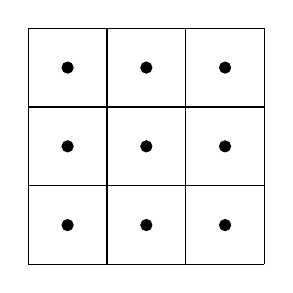
\begin{tikzpicture}
	\draw[step=1cm] (0, 0) grid (3cm, 3cm);
	\foreach \x in {0.5, 1.5, 2.5}
		\foreach \y in {0.5, 1.5, 2.5}
		{
			\filldraw (\x, \y) circle (2pt);
		}
\end{tikzpicture}
  \captionof{figure}{Grid based.}
  \label{fig:grid}
\end{minipage}%
\begin{minipage}{.5\textwidth}
  \centering
  \begin{tikzpicture}
	\draw (0, 0) .. controls (1, 1) and (1, -1.4) .. (3, 1);
	\draw (0, -1) .. controls (1, 0) and (1, -2.4) .. (3, 0);
	\draw (0, -2) .. controls (1, -1) and (1, -3.4) .. (3, -1);
	\filldraw (1, 0.05) circle (2pt);
	\filldraw (1.5, -1.1) circle (2pt);
	\filldraw (2, -1.95) circle (2pt);
\end{tikzpicture}
  \captionof{figure}{Particle based.}
  \label{fig:particle}
\end{minipage}
\end{figure}

\bigskip

The \textbf{Eulerian} way partitions the space into a grid and treats each cell as a localized region containing average data. As the size of the grid increases these localized cells become smaller, thus improving accuracy since the approximations of local values will be more accurate as well.

\bigskip

On the other hand, the using \textbf{Lagrangian} Coordinates we instead simulate individual particles and calculate their path and behavior while interacting with the environment.
At large scales this becomes more complex than the previous approach

\subsection{Restrictions}
The assumption of fluid \textbf{incompressibility} allows us to make use of the Navier-Stokes equations, which describe the flow of incompressible fluids, thus greatly simplífying the calculations needed.
Furthermore only \textbf{homogenous materials} are used; mixing of different fluids is not part of the simnulation.
\textbf{Viscosity} is not given as a property of the fluid, but rather implied by the use of limiting the diffusion rate.


\section{Pressure Field}

\subsection{Simple heuristics}

The equalization of pressure across the given region is almost instantaneous when adding pressure sources to it. For a simple heuristic simulation the following approach can be used:
\[ 
x_{i, j} = \frac{x_{i, j} + x_{i+1, j} + x_{i-1, j} + x_{i, j+1} + x_{i, j-1}}{5}
\]

This is adequate in hydrostatic problems, since there is no movement in the fluid.

\begin{lstlisting}
void Grid::diffuse()
{
	next_values[i][j] = (values[i][j] + values[i-1][j] + values[i+1][j] + values[i][j-1] + values[i][j+1]) / 5;
	values.swap(next_values);
}
\end{lstlisting}

\subsection{Problems}
For small areas, specifically the localozed region defined by the cells being averaged, this works, however since this is effectively an averaging kernel that goes through the entire grid there are bound to be losses in the global domain. 

\bigskip

Although this results in pressure losses and does not adhere to the conservation of energy we can still leverage it by stating that the global region of interest, the entire area being simulated, is not bounded nor constrained by anything, as if being a localized region of a greater system itself. Much like if one were to examine a volume of 1 $m^3$ of water in the ocean. If this system is large enough than no further problems will be caused by this discrepancy.

\bigskip

As mentioned in the restricions there are many physical effects not accounted for, especially at the edges and in the corners of the grid, however since the distribution of pressure is defined as an average of a given cell and its neighbours' these cases must be handeled regardless.

\bigskip

Possible solutions are to limit the space that the kernel iterates through and leave a 1 cell thick \textit{border} on all sides, and or change the size (consequently the shape) of the kernel making it a $3x3$ square, which would get eliminate the problems caused by the corners.

\subsection{Diffusion}

When the velocity flow field is taken into account the issue of pressure distribution becomes much harder. This change with respect to time can be described by differentioal equations, but these would introduce much more calculations and solving for each individual cell is costly.

\begin{center}
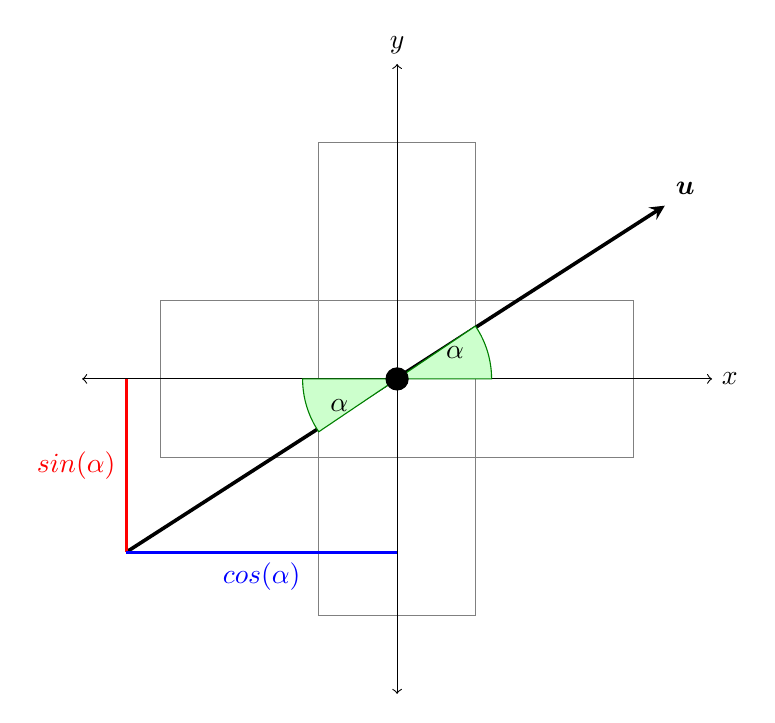
\begin{tikzpicture}[scale=2]
	%\filldraw[lightgray] (0, 0) rectangle (1, 1);
	\draw[gray] (0, 0)	rectangle (1, 1);
	\draw[gray] (0, 1)	rectangle (1, 2);
	\draw[gray] (-1, 0) rectangle (0, 1);
	\draw[gray] (0, -1) rectangle (1, 0);
	\draw[gray] (1, 0)	rectangle (2, 1);

	\draw[<->] (-1.5, 0.5) -- (2.5, 0.5) node[right]{$x$};
	\draw[<->] (0.5, -1.5) -- (0.5, 2.5) node[above]{$y$};
	
	\draw[line width=1.3pt,-stealth](-1.22, -0.6)--(2.2, 1.6) node[anchor=south west]{$\boldsymbol{u}$};
	
	\draw[red,very thick] (-1.22, -0.6) -- (-1.22, 0.5) node[midway, left]{$sin(\alpha)$};
	\draw[blue,very thick] (-1.22, -0.6) -- (0.5, -0.6) node[midway, below]{$cos(\alpha)$};
	
	\filldraw[fill=green!20!white, draw=green!50!black] (0.5, 0.5) -- (1.1, 0.5) arc (0:34:0.6) -- cycle node[midway, right]{$\alpha$};
	\filldraw[fill=green!20!white, draw=green!50!black] (0.5, 0.5) -- (-0.1, 0.5) arc (180:214:0.6) -- cycle node[midway, left]{$\alpha$};
	
	\filldraw (0.5, 0.5) circle (2pt);
\end{tikzpicture}
\end{center}

So instead we alter the previous calculations and now include information about the vector field as well. The flow in each localized region is described by a single vector, whose direction and magnitude correspond to the fluid's flow direction and speed respectively.

\bigskip

The direction of flow also determines how the pressure changes, so any alterations in the flow velocity field will cause a change in pressure distribution.
Instead of using conventional averages we use weighted averages where the weights are the distance of grids located in the path of fluid flow from the vector itself.
The \textit{closer} a vector is to a grid cell the more significantly it contributes to the change in pressure. 

\bigskip

These distances are the $sin(\alpha)$ and $cos(\alpha)$ in the $y$ and $x$ directions respectively. After normalizing the vector there is no need to calculate these values and we can just use the $x$ and $y$ coordinates of the subsequent unit vector instead.

\bigskip

Cells on the $x$ axis are weighted with $sin(\alpha)$ and grid cells located on the $y$ axis are multiplied by $cos(\alpha)$. The calculation is done in the following manner:

\[
	vec = \text{normalized vector at }cell_{i, j}
\]

\[
	cell_{i, j} = \begin{cases}
	vec.x \cdot cell_{i+1, j} + vec.y \cdot cell_{i, j-1}, & x > 0, y > 0 \\
	vec.x \cdot cell_{i-1, j} + (-1)\cdot vec.y \cdot cell_{i, j-1}, & x > 0, y < 0 \\
	(-1) \cdot vec.x \cdot cell_{i-1, j} + (-1) \cdot vec.y \cdot cell_{i, j+1}, & x < 0, y < 0 \\
	(-1) \cdot vec.x \cdot cell_{i-1, j} + vec.y \cdot cell_{i, j+1}, & x < 0, y > 0
	\end{cases}
\]

And the following function listed below implements this mechanism of diffusion.

\pagebreak

\begin{lstlisting}
void Grid::diffuse()
{
    Vec2 vec;
    for(int i = 1; i < gridSize-1; i++){
        for(int j = 1; j < gridSize-1; j++){
            vec = velocityField[i][j].normalize();
            double sum = 0;
            if(vec.x > 0 && vec.y > 0){
                sum = (vec.y)*values[i+1][j] + (vec.x)*values[i][j-1];
            }
            else if(vec.x > 0 && vec.y < 0){
                sum = (-vec.y)*values[i-1][j] + (vec.x)*values[i][j-1];
            }
            else if(vec.x < 0 && vec.y < 0){
                sum = (-vec.y)*values[i-1][j] + (-vec.x)*values[i][j+1];
            }
            else if(vec.x < 0 && vec.y > 0){
                sum = (vec.y)*values[i+1][j] + (-vec.x)*values[i][j+1];
            }

            if(std::abs(vec.x) + std::abs(vec.y) == 0) next_values[i][j] = 0;
            else next_values[i][j] = sum/(std::abs(vec.x) + std::abs(vec.y));
        }
    }
    values.swap(next_values);
}
\end{lstlisting}

\section{Velocity Flow Field}

This property defines the local velocities at which the fluid in a given are moves and is typically modelled as a vector field, which is free from divergence. Without divergence we adhere to our aforementioned rules of incompressibility and conservation of mass.

Each grid cell in our program has a corresponding vector in its center indicating the direction and velocity of the flow in the region.

\subsection{Static advection}

External forces contribute greatly to the advection or change in the flow of a fluid, however without them the flow is considered static (or hydrostatic in the case of water). In such cases we simulate advection the same way as in the averaging of the pressure field, but with the velocity vectors.

\[
vec_{i,j} = \frac{vec_{i,j} + vec_{i+1,j} + vec_{i-1,j} + vec_{i,j+1} + vec_{i,j-1}}{5}
\]

If the length of a vector goes below a certain $\epsilon$ value then it is considered a null vector, where the flow is zero.

\begin{lstlisting}
void Grid::advect()
{
    for(int i = 1; i < gridSize-1; i++){
        for(int j = 1; j < gridSize-1; j++){
            next_velocityField[i][j] = (velocityField[i][j] + velocityField[i-1][j] + velocityField[i+1][j] + velocityField[i][j-1] + velocityField[i][j+1])*(1/5.0);
            if(next_velocityField[i][j].length() < 0.1) next_velocityField[i][j] = Vec2(0, 0);
        }
    }
    velocityField.swap(next_velocityField);
}
\end{lstlisting}

\subsection{Dynamic advection}

Since the simulation is performed in real-time it allows the user to interact with the fluid, making it possible to add extra pressure to local regions and modify the flow field by moving the mouse cursor.

\bigskip

First we must store the mouse's $x$ and $y$ positions in the event of a click and add it to and array of length $N$. This array serves as a moving window to help in the averaging of the cursor's speed and direction. The previous and the current position of the mouse would be sufficient enough to determine the speed and direction, howerver with only these two values the result would look choppy and discontinous, since the pixels themselves are arranged in a grid-like fashion results in the aforementioned calculations would incur a vector either parallel to an axis or angeled at $45^{\circ}$ at all times.

\bigskip

\begin{lstlisting}
void Screen::mousePressEvent(QMouseEvent *event)
{
    mousePos.x = event->pos().x();
    mousePos.y = event->pos().y();

    path.push_back(QPoint(mousePos.x, mousePos.y));
    cursorDirection.x = 0;
    cursorDirection.y = 0;
}
\end{lstlisting}

\bigskip

Then at every instance we register a mouse movement we store the current position of the cursor in the array, if it were to fil up, the values at the end, or in other words the oldest recorded position will be discarded.

\begin{lstlisting}
void Screen::mouseMoveEvent(QMouseEvent *event)
{
    Vec2 currentPos = Vec2(event->pos().x(), event->pos().y());
    Vec2 speed = currentPos - mousePos;
    mousePos = currentPos;
    speed.y *= -1;
    cursorDirection = speed;
    path.push_back(QPoint(mousePos.x, mousePos.y));
    index = (index+1) % wndSize;
    directions[index] = cursorDirection;
}
\end{lstlisting}

\bigskip

Finally we average out these values resulting in a vector representing the speed and direction of movement of the cursor. Since the average is \textit{moving} this averaged vector will follow the mouse's true speed and direction quite smoothly.

\begin{lstlisting}
Vec2 smoothDir(0, 0);
for(Vec2 v : directions){
    smoothDir = smoothDir + v;
}
smoothDir = smoothDir * (1/(double)wndSize);
\end{lstlisting}

\bigskip

Each time the screen is rendered we must calculate this moving average and using the mouse coordinates map it to our 2 dimensional grid in order to modify the flow velocity vector located in the correct region.

\begin{lstlisting}
i = event->pos().y()/(sizeY/gridSize)
j = event->pos().x()/(sizeX/gridSize)
velocityField[i][j] = smoothDir;
\end{lstlisting}

\section{Displaying the vector field}

After each individual vector in the flow velocity field has been calculated the user can chose whether to visualize them or not with the following function.

\begin{lstlisting}
void Grid::paintEvent(QPaintEvent *event)
{
    ...
    
    for(int i = 0; i < gridSize; i++){
        for(int j = 0; j < gridSize; j++){
            painter.translate(j*cellSize + cellSize/2.0, i*cellSize + cellSize/2.0);
            painter.scale(1, -1);
            QLineF line(0, 0, velocityField[i][j].x, velocityField[i][j].y);
            
            ...
        }
    }
}
\end{lstlisting}

Drawing the head of each vector is a bit tricky, but it can be achieved with a little calculation.

\begin{lstlisting}
	
	...
	
	painter.setPen(Qt::red);
    painter.drawLine(line);
            
	QPolygon head;
	int h = 10;
    double len = sqrt(velocityField[i][j].x*velocityField[i][j].x + velocityField[i][j].y*velocityField[i][j].y);
    
    head << QPoint((velocityField[i][j].x - velocityField[i][j].y/len*3), (velocityField[i][j].y + velocityField[i][j].x/len*3)) 
    
    << QPoint((velocityField[i][j].x + velocityField[i][j].y/len*3), (velocityField[i][j].y - velocityField[i][j].x/len*3))
    
    << QPoint(velocityField[i][j].x + h * (velocityField[i][j].x/len), velocityField[i][j].y + h * (velocityField[i][j].y/len));
    
    painter.setPen(Qt::green);
    painter.drawPolygon(head);
    painter.resetTransform();
    
    ...
    
\end{lstlisting}

After this the whole of the velocity flow field can be displayed in its full form, their lengths  indicating the speed of the flow in that specific localized region.

\pagebreak

\section{Conclusion}

The following snapshots have been taken while running the simulation. The vector field is set to visible and fluid pressure is distinguished by its red to light green gradient.

\begin{figure}[h!]
  \centering
  \begin{subfigure}[b]{0.4\linewidth}
    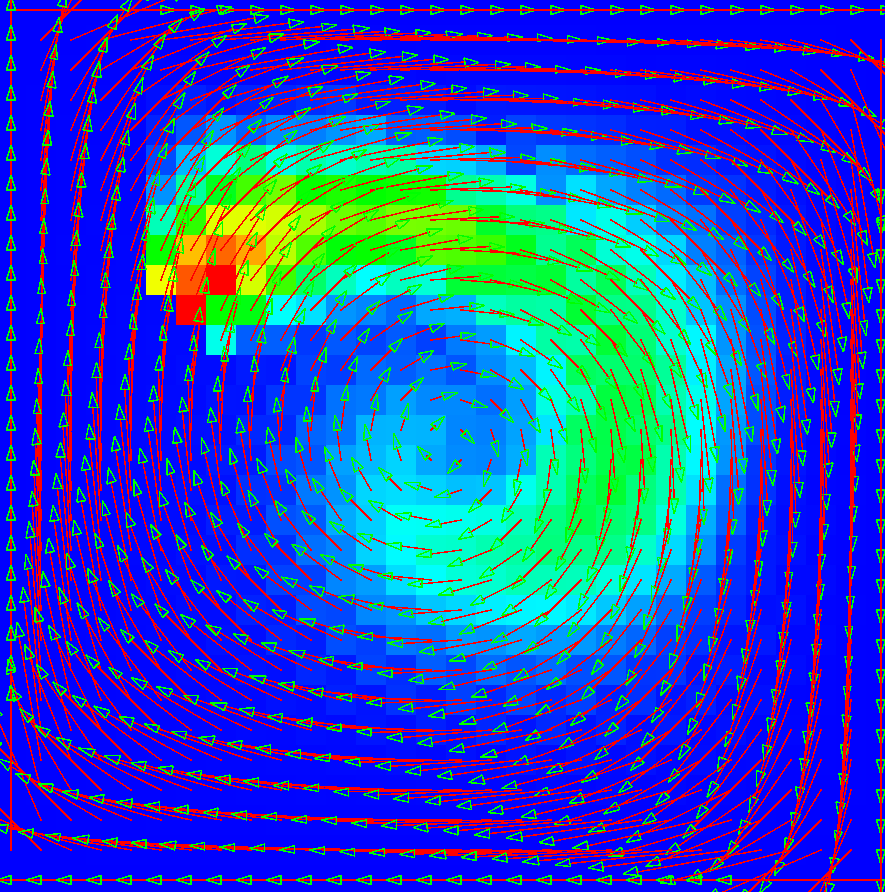
\includegraphics[width=\linewidth]{images/sim2.png}
    \caption{Visible pressure gradient.}
  \end{subfigure}
  \begin{subfigure}[b]{0.4\linewidth}
    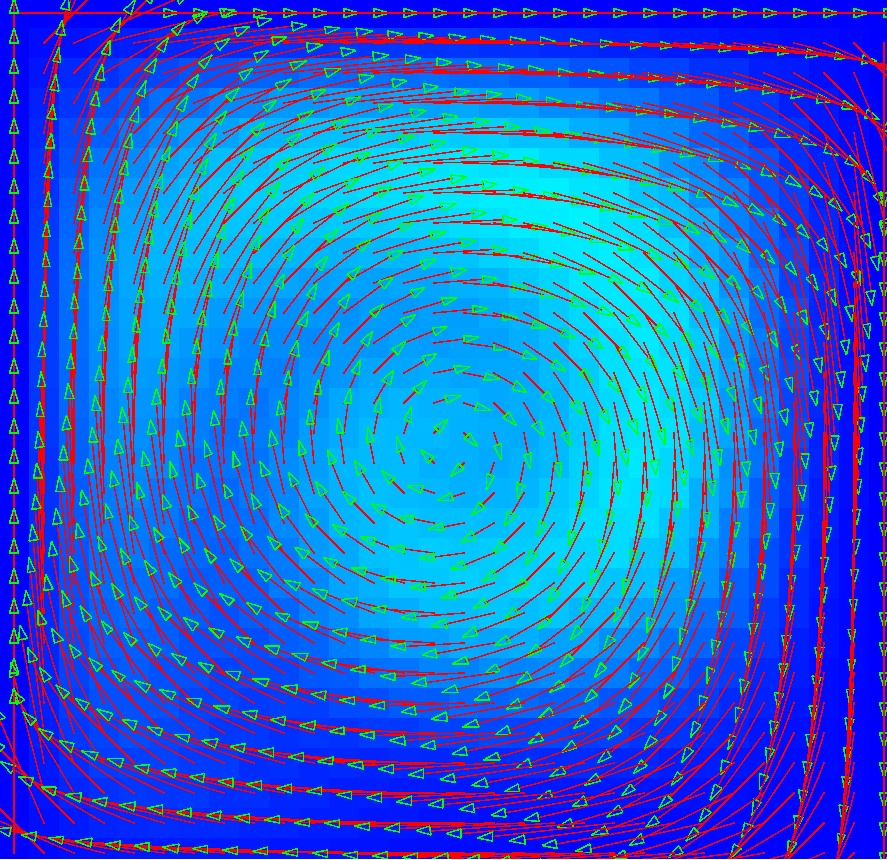
\includegraphics[width=\linewidth, height=55.3mm]{images/sim1.png}
    \caption{Diffusion.}
  \end{subfigure}
  \caption{Circular diffusion with velocity flow field.}
  \label{fig:circular}
\end{figure}



\begin{figure}[h!]
  \centering
  \begin{subfigure}[b]{0.4\linewidth}
    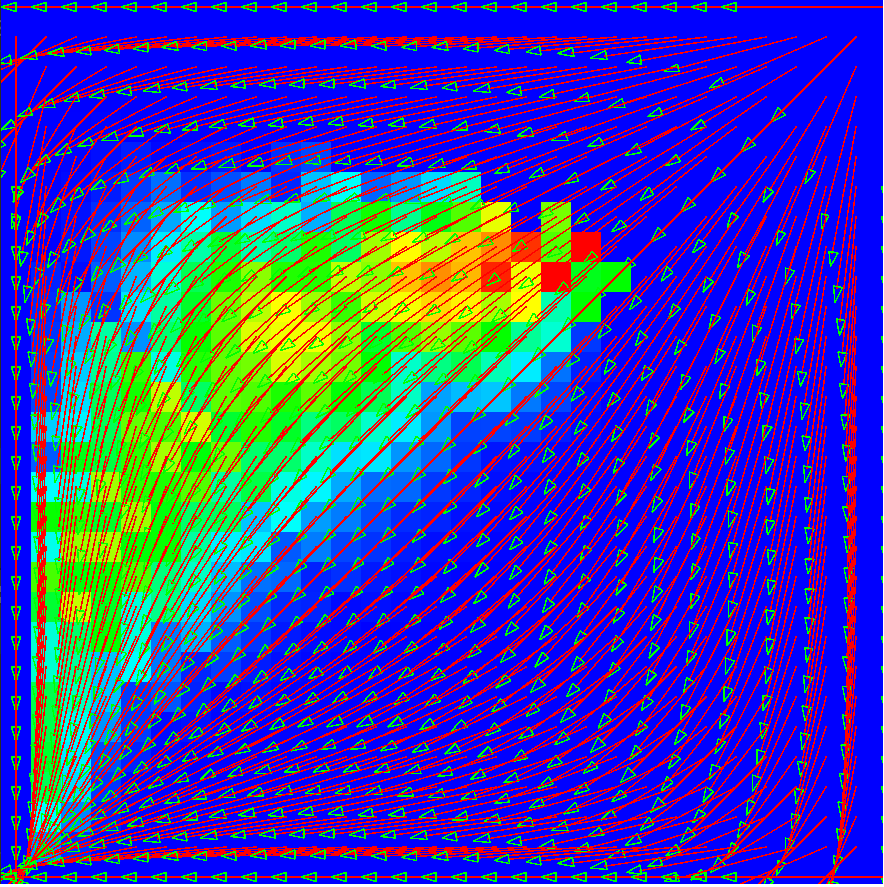
\includegraphics[width=\linewidth]{images/sim3.png}
    \caption{Flow towards left lower corner.}
  \end{subfigure}
  \begin{subfigure}[b]{0.4\linewidth}
    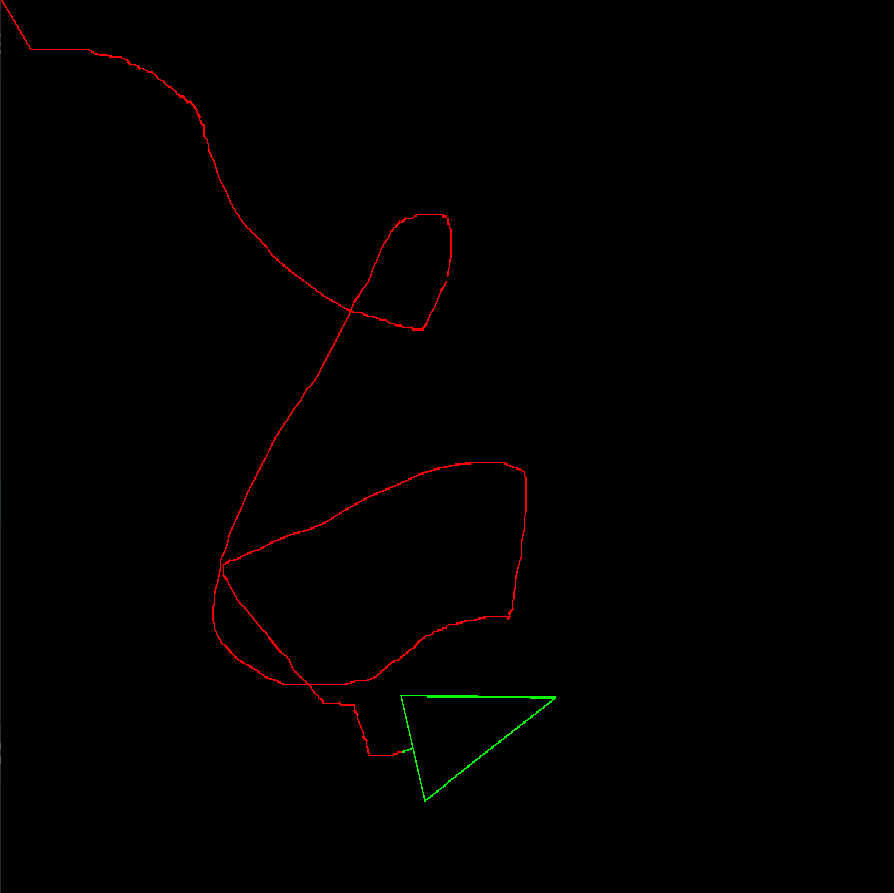
\includegraphics[width=\linewidth]{images/cursor.png}
    \caption{Recorded cursor direction and intensity.}
  \end{subfigure}
  \caption{Diffusion and dynamic advection algorithm visualizer.}
  \label{fig:left flow with cursor follow}
\end{figure}


\end{document}